%
% File ACL2016.tex
%

\documentclass[11pt]{article}
\usepackage{acl2016}
\usepackage{times}
\usepackage{latexsym}
\usepackage{graphicx}
\usepackage{multirow}

%\aclfinalcopy % Uncomment this line for the final submission
%\def\aclpaperid{***} %  Enter the acl Paper ID here

% To expand the titlebox for more authors, uncomment
% below and set accordingly.
% \addtolength\titlebox{.5in}    

\newcommand\BibTeX{B{\sc ib}\TeX}
\newcommand*\rot{\rotatebox{90}}

\title{Inferring Topic Domains from Topics in Newspaper and Web Data}

% Author information can be set in various styles:
% For several authors from the same institution:
% \author{Author 1 \and ... \and Author n \\
%         Address line \\ ... \\ Address line}
% if the names do not fit well on one line use
%         Author 1 \\ {\bf Author 2} \\ ... \\ {\bf Author n} \\
% For authors from different institutions:
% \author{Author 1 \\ Address line \\  ... \\ Address line
%         \And  ... \And
%         Author n \\ Address line \\ ... \\ Address line}
% To start a seperate ``row'' of authors use \AND, as in
% \author{Author 1 \\ Address line \\  ... \\ Address line
%         \AND
%         Author 2 \\ Address line \\ ... \\ Address line \And
%         Author 3 \\ Address line \\ ... \\ Address line}
% If the title and author information does not fit in the area allocated,
% place \setlength\titlebox{<new height>} right after
% at the top, where <new height> can be something larger than 2.25in
\author{Roland Schäfer\\
	    Freie Universität Berlin\\
	    Habelschwerdter Allee 45\\
	    14196 Berlin, Germany\\
	    {\tt roland.schaefer@fu-berlin.de}
	  \And
	Felix Bildhauer\\
  	Institut für Deutsche Sprache\\
  	R5, 6--13\\
  	68161 Mannheim, Germany\\
  {\tt bildhauer@ids-mannheim.de}}

\date{}

\begin{document}

\maketitle

\begin{abstract}
\end{abstract}

\section{Introduction}

In this paper, we describe preliminary encouraging results from an ongoing experiment wherein we classify large unstructured text corpora (such as web corpora) by \textit{topic domain}.
While topics modelling . . . linguists are often interested in high-level classifications such as genre, register, or topic domain.


Why topic domain?

Automatic meta data: desirable not JUST for web data.

Short comments on register scene and poor results in recent Globbe paper.

Mention corpus comparison as important field: Kilgarriff, WCC, "Biemann et al."

\section{Gold standard Data}

Corpora \cite{KupietzEa2010}, SchäBi 2012, Schä 2015

Annotation scheme: Sharoff; mention that it was developed in repeated annotation processes based on annotator feedback; mention that design goal was roughly 10 to 20 topic domains

\section{Experiment Setup}

Pre-processing

Algorithms (LSI/LDA)

Gold and plus versions

Filters and lexicon thresholds

Numbers of topics

SVM vs. Trees; SVM kernel selection

Elimination of very small topic domains

\section{Results}

\begin{figure*}[ht]
  \centering
  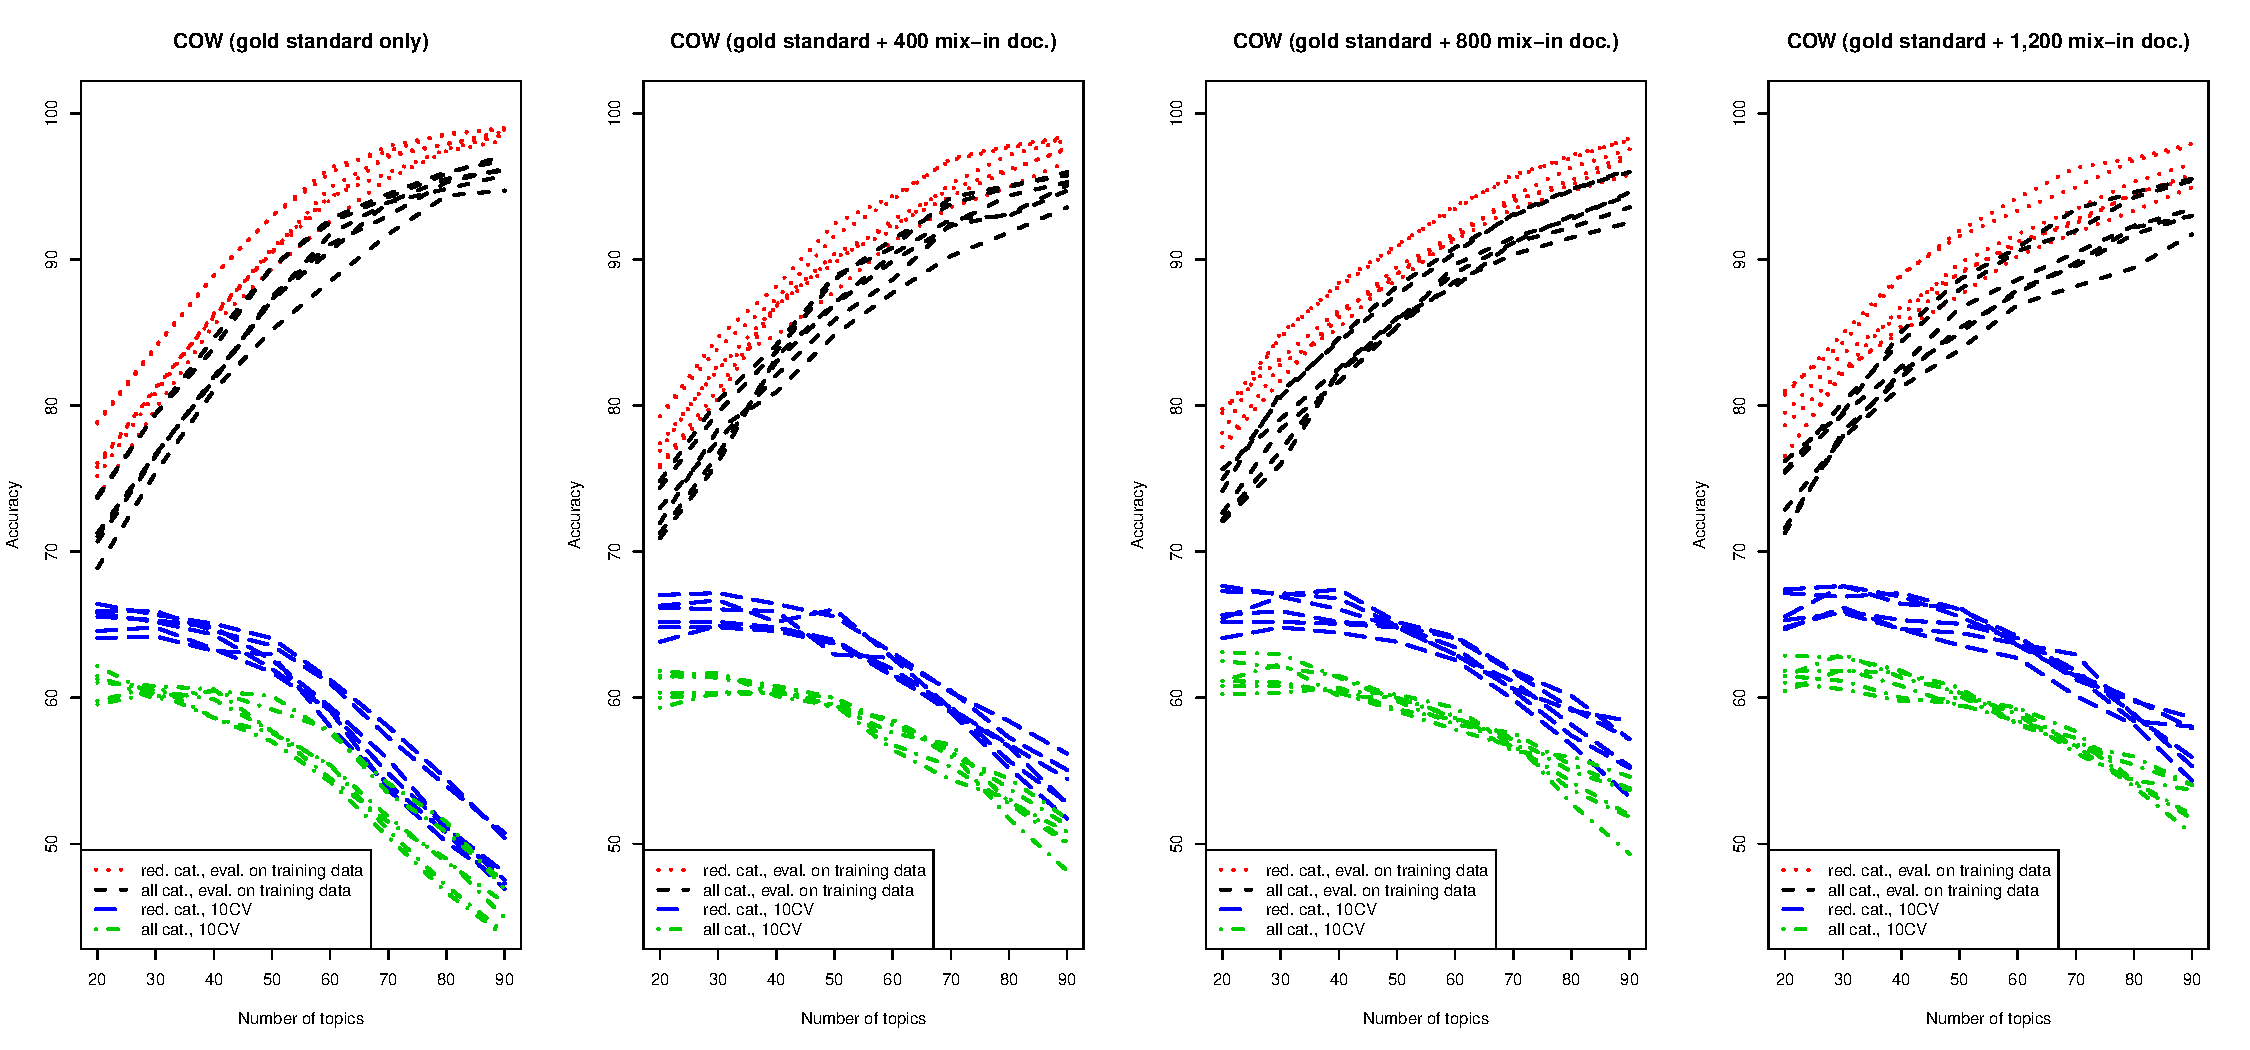
\includegraphics[width=\textwidth]{graphics/cow.pdf}
  \caption{Accuracy with different numbers of topics for COW-only dataset}
  \label{fig:cow}
\end{figure*}

Figure~\ref{fig:cow} shows the classification accuracy for 20 to 90 LSI topics.
Each line corresponds to one sub-experiment, and the lines form well distinguishable bands.
The highest accuracy is achieved with a reduced set of topic domains when the evaluation is performed on the training data (upper six dotted lines).
The full set of topic domains leads to a drop in accuracy of about 5\% (six upper dashed lines).
The two lower bands show the classification accuracy in a 10-fold cross-validation (10CV), again with the reduced set of topic domains faring roughly 5\% better.
While a higher number of topics improves results on the training data, the accuracy in the cross-validation drops.
Too large numbers of topics obviously allows the method to pick up idiosyncratic features of single documents or very small clusters, leading to extreme overtraining.
The four panels show results based of different topic models.
Panel (a) uses a topic model inferred only from the 870 gold standard documents.
Results in panel (b) through (d) are based on topic models inferred on larger data sets (larger in increments of roughly 50\% of the original number of documents) in order to stabilize the topic distribution.
In the experiment reported in panel (d), for example, 1,200 documents were added to the 870 gold standard documents.
While the overtraining effect is alleviated by mixing in more documents, the maximum achieved accuracy does not significantly improve.
We continued the experiment (further results not shown here), mixing in up to 8,000 additional documents with no significant change compared to panel (d) in Figure~\ref{fig:cow}.
We consider the maximum 10CV accuracy with the reduced set of topic domains most informative w.\,r.\,t.\ the potential quality of the classifier, and we report it in Table~\ref{tab:quality}.

\begin{table*}[ht]
  \centering
  \resizebox{\textwidth}{!}{\begin{tabular}{|lrllrrrrr|}
    \hline
    \textbf{Corpus} & \textbf{Mixed-in} & \textbf{Filters} & \textbf{Attribute} & \textbf{Topics} & \textbf{Accuracy} & \textbf{Precision} & \textbf{Recall} & \textbf{F-Measure} \\
    \hline
    COW & $\sim$3,200 & set 2 & token & 20 & 68.765\% & 0.688 & 0.688 & 0.674 \\
    DeReKo & $\sim$3,600 & set 2 & lemma + POS & 40 & 72.162\% & 0.716 & 0.722 & 0.686 \\
    COW + DeReKo & 0 & set 2 & lemma + POS & 30 & 51.872\% & 0.431 & 0.519 & 0.417 \\ 
    \hline
  \end{tabular}}
  \caption{Evaluation at best achievable accuracy with the reduced set of topic domains in 10-fold cross-validation; Precision, Recall, and F-Measure are weighted averages across all categories}
  \label{tab:quality}
\end{table*}

\begin{figure*}[ht]
  \centering
  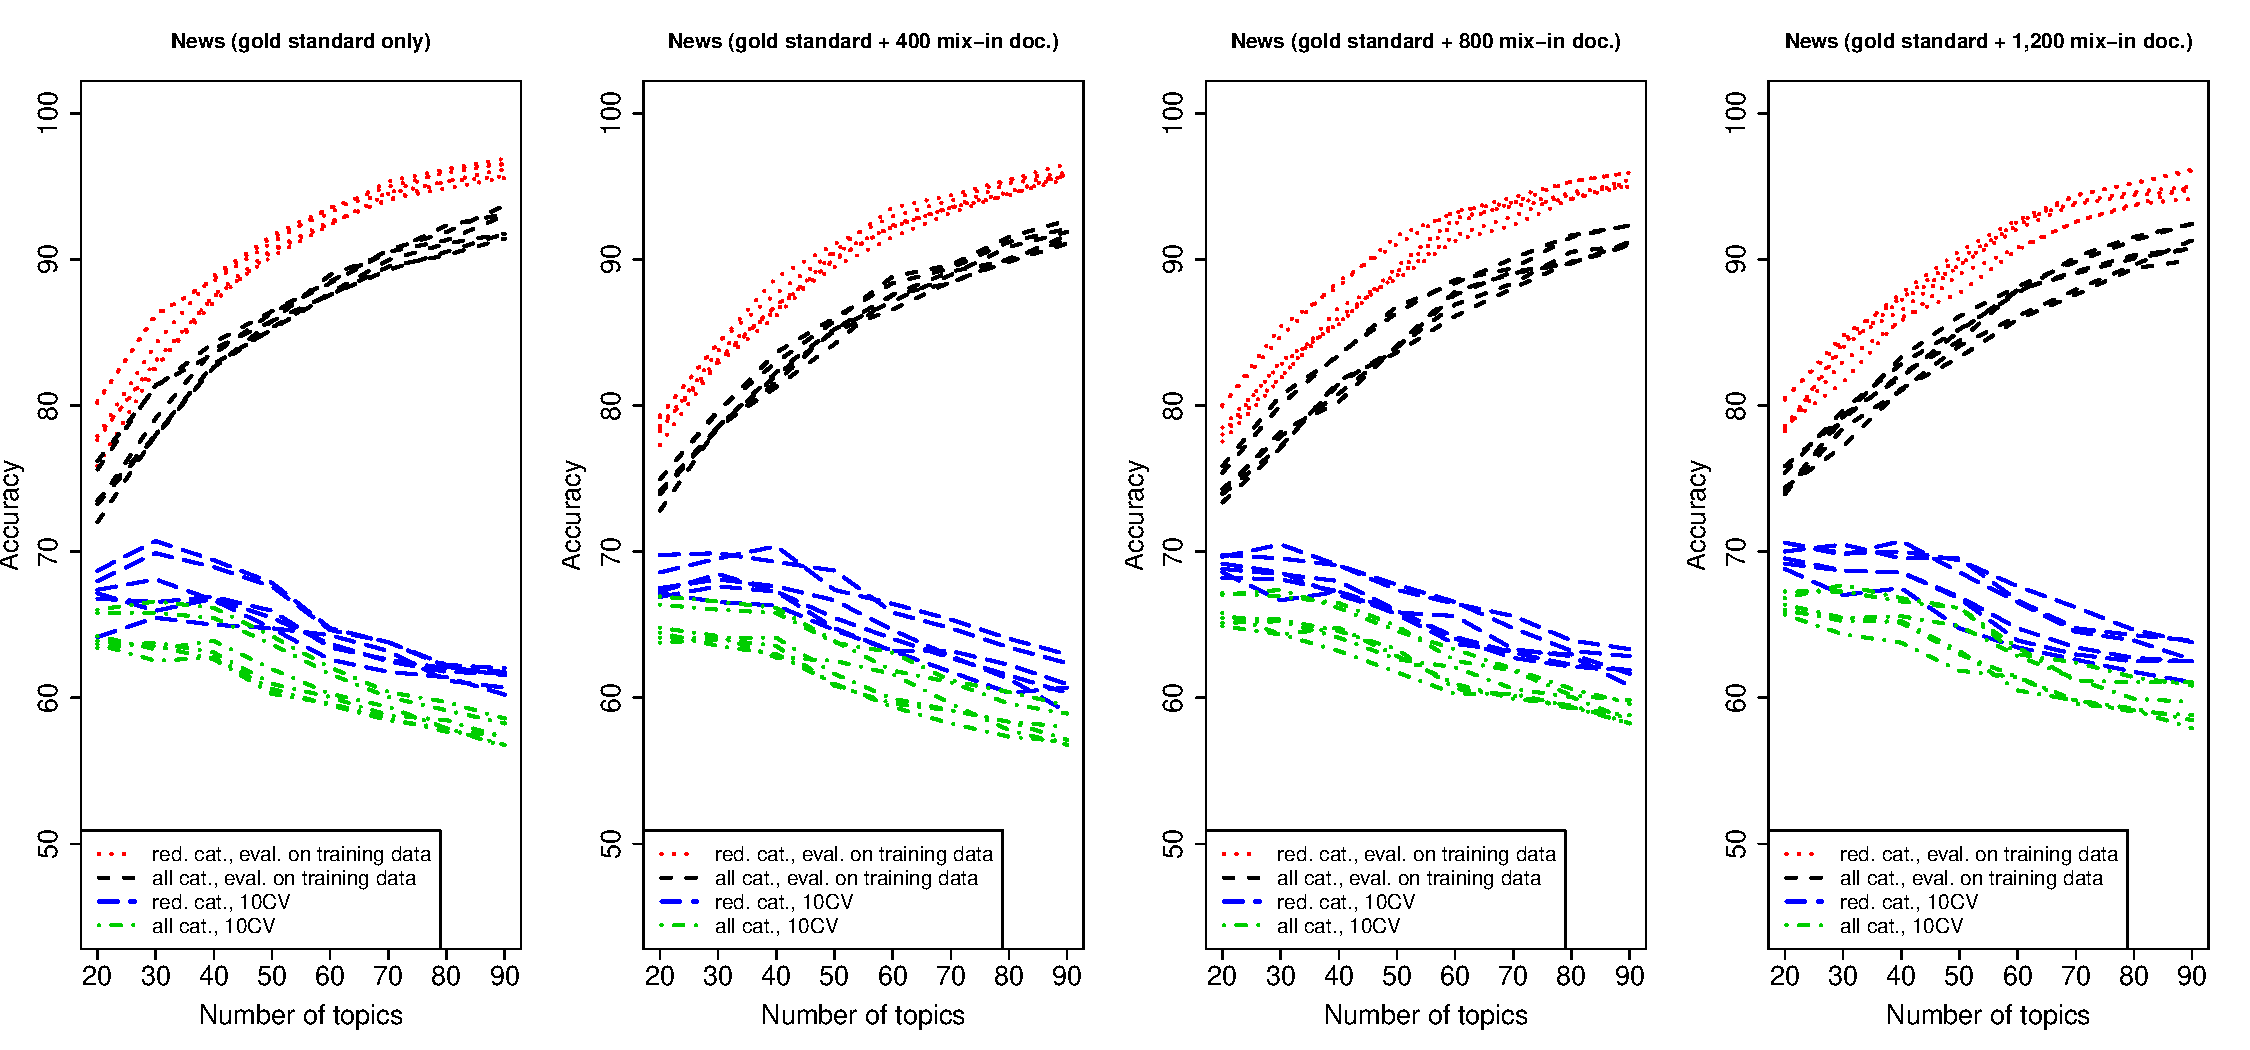
\includegraphics[width=\textwidth]{graphics/dereko.pdf}
  \caption{Accuracy with different numbers of topics for DeReKo-only dataset}
  \label{fig:dereko}
\end{figure*}

A parallel plot for the DeReKo data is shown in Figure~\ref{fig:coreko}, maximally best results are also given in Table~\ref{tab:quality}.
The picture is essentially the same as for the COW data set.
The added accuracy (3.397\% according to Table~\ref{tab:quality}) is a side effect of the more skewed distribution of topic domains in the DeReKo gold standard data.
The $\kappa$ statistic for the COW and DeReKo results from Table~\ref{tab:quality} of $\kappa_{\textrm{\tiny COW}}=0.575$ and $\kappa_{\textrm{\tiny DeReKo}}=0.569$ show that achieving a higher accuracy for the COW data is actually harder in comparison with the DeReKo data.

\begin{figure*}[ht]
  \centering
  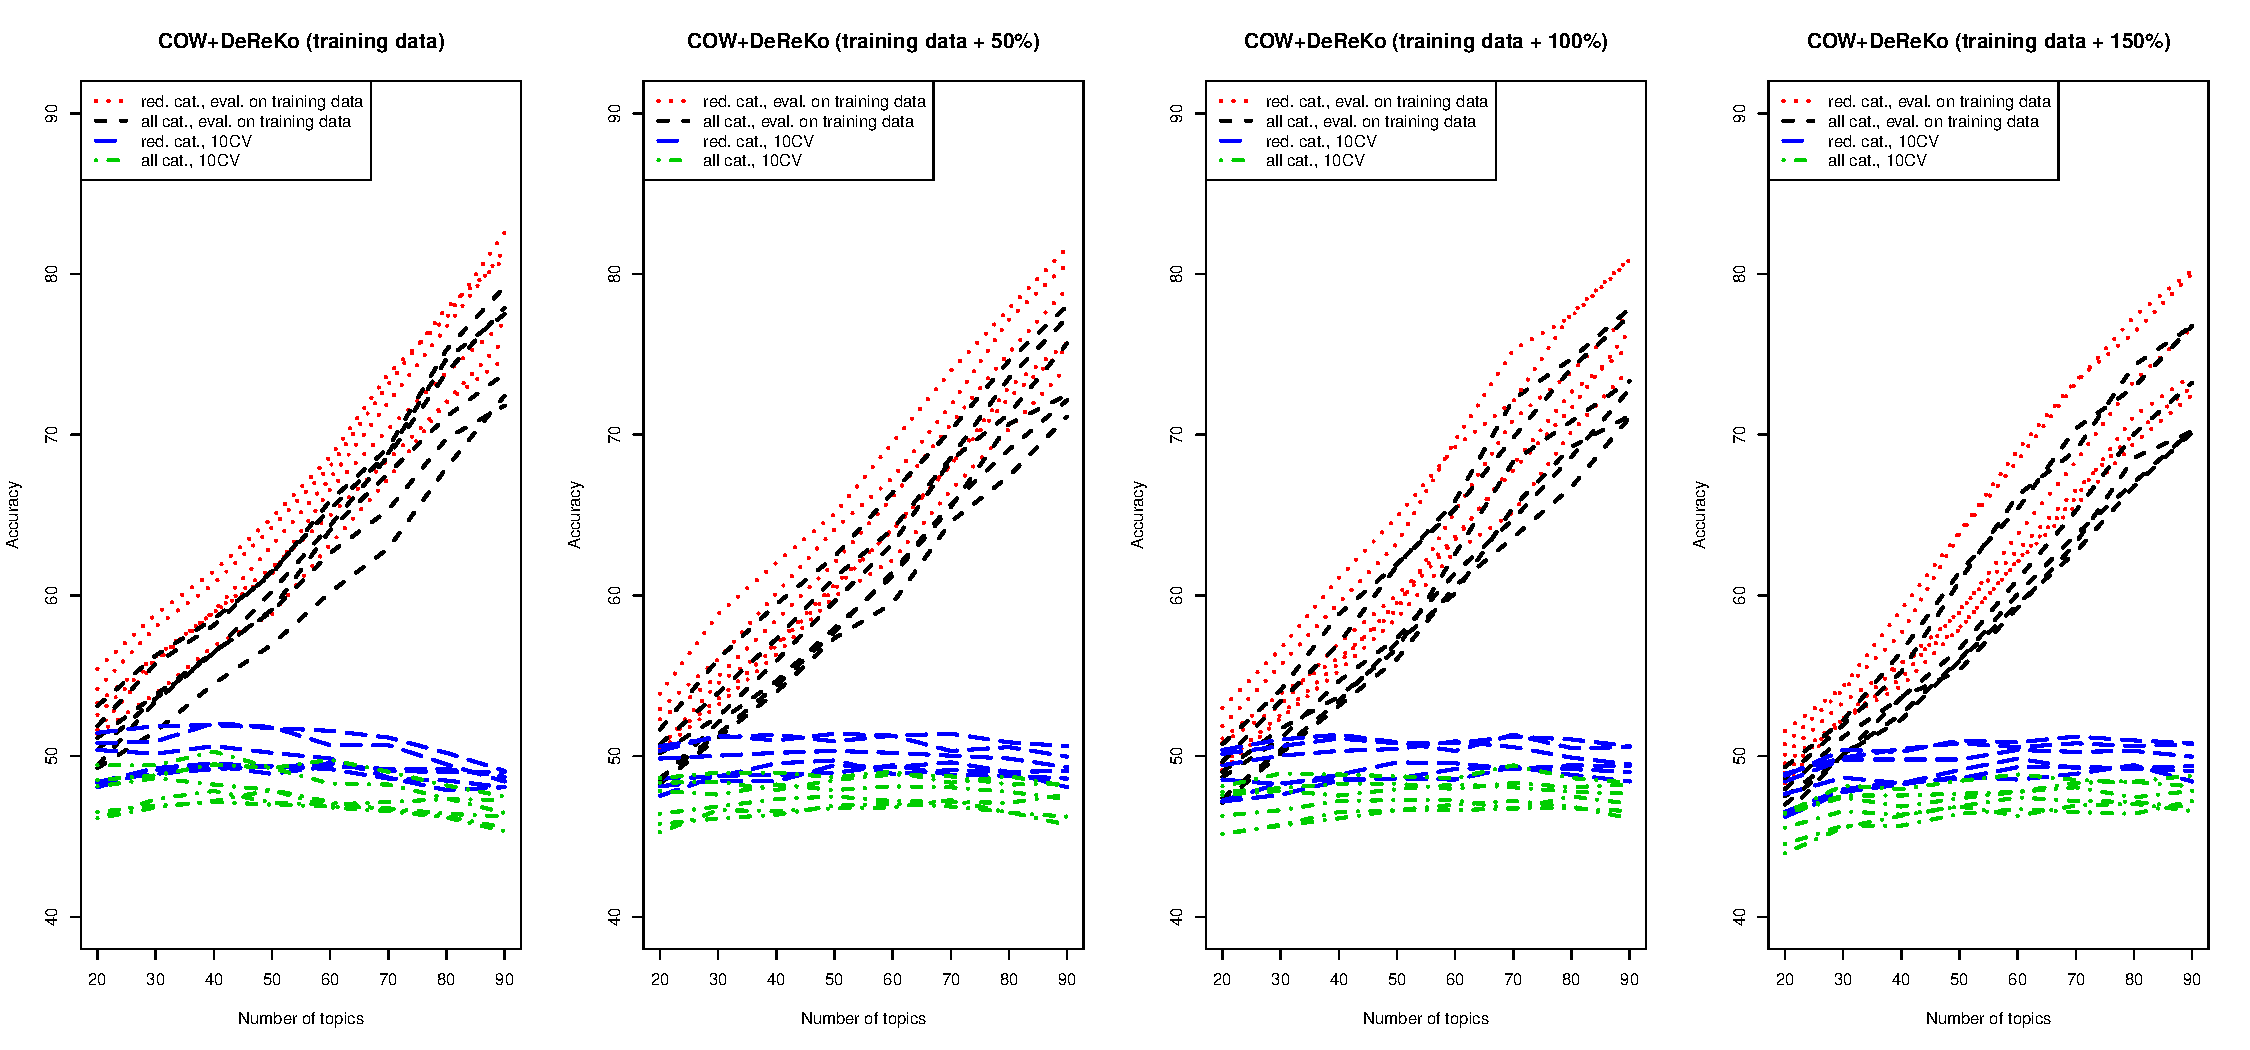
\includegraphics[width=\textwidth]{graphics/coreko.pdf}
  \caption{Accuracy with different numbers of topics for COW+DeReKo dataset}
  \label{fig:coreko}
\end{figure*}

When the COW and DeReKo data are pooled, however, quality drops below any acceptable level, cf.\ Figure~\ref{fig:coreko} and Table~\ref{tab:quality}.
Mixing in more documents improves the evaluation results on the training data, but the 10CV results---which give us a more realistic idea of the real-world performance of the classifier---remains steady at around 50\%.
This is remarkable because larger training data sets should lead to increased, not degraded accuracy.
While a deeper analysis of the LSI topic distributions remains to be undertaken, it becomes clear what causes these below average results on the side of the SVM classifier when looking at the confusion matrices, cf.\ Table~\ref{tab:confusion}.
While the COW data set show a less than perfect but 

\begin{table*}[ht]
  \centering
  \resizebox{0.33\textwidth}{!}{\begin{tabular}{|llcccccccc|}
    \hline
    \multicolumn{2}{|c}{\textbf{COW}} & \multicolumn{8}{c|}{\textbf{Classified}} \\
     && \rot{\textbf{PolSoc~}} & \rot{\textbf{Busi}} & \rot{\textbf{Life}} & \rot{\textbf{Arts}} & \rot{\textbf{Public~}} & \rot{\textbf{Law}} & \rot{\textbf{Beliefs~}} & \rot{\textbf{Hist}} \\
   \hline
   \multirow{8}{*}{\rot{\textbf{Annotated}}} & \textbf{PolSoc}  & \textbf{26} &  12 &  10 &   1 &   1 &   0 &   1 &   0 \\ 
     & \textbf{Busi}    &  5 & \textbf{105} &  40 &   7 &   1 &   2 &   1 &   1 \\ 
     & \textbf{Life}    &  3 &  14 & \textbf{286} &   6 &   4 &   1 &   1 &   1 \\ 
     & \textbf{Arts}    &  3 &   2 &  36 &  \textbf{78} &   1 &   0 &   2 &   6 \\ 
     & \textbf{Public}  &  0 &   3 &  11 &   0 &   \textbf{9} &   1 &   0 &   0 \\ 
     & \textbf{Law}     &  3 &   9 &   8 &   0 &   1 &   \textbf{8} &   0 &   0 \\ 
     & \textbf{Beliefs} &  4 &   3 &  11 &   6 &   1 &   0 &  \textbf{30} &   1 \\ 
     & \textbf{Hist}    &  9 &   0 &   9 &   7 &   1 &   1 &   2 &  \textbf{15} \\ 
     \hline
 \end{tabular}}~~\resizebox{0.32\textwidth}{!}{\begin{tabular}{|llcccccccc|}
    \hline
     \multicolumn{2}{|c}{\textbf{DeReKo}} & \multicolumn{8}{c|}{\textbf{Classified}} \\
     && \rot{\textbf{PolSoc~}} & \rot{\textbf{Busi}} & \rot{\textbf{Life}} & \rot{\textbf{Arts}} & \rot{\textbf{Public~}} & \rot{\textbf{Law}} & \rot{\textbf{Beliefs~}} & \rot{\textbf{Hist}} \\
    \hline
    \multirow{8}{*}{\rot{\textbf{Annotated}}} & \textbf{PolSoc}  & \textbf{222} &   5 &  41 &   0 &   8 &   0 &   0 &   0 \\
    & \textbf{Busi}    &  19 &  \textbf{25} &   8 &   0 &   1 &   0 &   0 &   0 \\ 
    & \textbf{Life}    &  27 &   1 & \textbf{321} &   0 &   1 &   0 &   0 &   0 \\ 
    & \textbf{Arts}    &   2 &   0 &  29 &   \textbf{5} &   0 &   0 &   0 &   0 \\ 
    & \textbf{Public}  &  41 &   0 &  27 &   0 &  \textbf{31} &   0 &   0 &   0 \\ 
    & \textbf{Law}     &  10 &   0 &   0 &   0 &   0 &   \textbf{0} &   0 &   0 \\ 
    & \textbf{Beliefs} &   0 &   0 &   3 &   0 &   0 &   0 &   \textbf{0} &   0 \\ 
    & \textbf{Hist}    &   2 &   0 &   7 &   0 &   1 &   0 &   0 &   \textbf{0} \\ 
   \hline
 \end{tabular}}~~\resizebox{0.315\textwidth}{!}{\begin{tabular}{|llccccccccc|}
    \hline
     \multicolumn{2}{|c}{\textbf{Joint}} & \multicolumn{9}{c|}{\textbf{Classified}} \\
     && \rot{\textbf{PolSoc~}} & \rot{\textbf{Busi}} & \rot{\textbf{Medical~}} & \rot{\textbf{Life}} & \rot{\textbf{Arts}} & \rot{\textbf{Public~}} & \rot{\textbf{Law}} & \rot{\textbf{Beliefs~}} & \rot{\textbf{Hist}} \\
    \hline
    \multirow{9}{*}{\rot{\textbf{Annotated}}} & \textbf{PolSoc}   & \textbf{199} &   7 &   0 & 109 &   0 &  12 &   0 &   0 &   0 \\ 
    & \textbf{Busi}     &  18 &  \textbf{23} &   0 & 172 &   0 &   2 &   0 &   0 &   0 \\ 
    & \textbf{Medical}  &   6 &   0 &   \textbf{0} &  29 &   0 &   1 &   0 &   0 &   0 \\ 
    & \textbf{Life}     &  25 &   4 &   0 & \textbf{632} &   0 &   5 &   0 &   0 &   0 \\ 
    & \textbf{Arts}     &   2 &   2 &   0 & 160 &   \textbf{0} &   0 &   0 &   0 &   0 \\ 
    & \textbf{Public}   &  46 &   2 &   0 &  56 &   0 &  \textbf{19} &   0 &   0 &   0 \\ 
    & \textbf{Law}      &   8 &   0 &   0 &  31 &   0 &   0 &   \textbf{0} &   0 &   0 \\ 
    & \textbf{Beliefs}  &   0 &   0 &   0 &  59 &   0 &   0 &   0 &   \textbf{0} &   0 \\ 
    & \textbf{Hist}     &   4 &   0 &   0 &  50 &   0 &   0 &   0 &   0 &   \textbf{0} \\ 
    \hline
 \end{tabular}}
  \caption{Confusion matrices for the best achievable results on the COW (a), DeReKo (b), and joint (c) data sets as reported in Table~\ref{tab:quality}}
  \label{tab:confusion}
\end{table*}

\section{Conclusions and Outlook}

The results presented here are preliminary, but highly encouraging (over 90\% accuracy on training data and over 70\% accuracy in cross-validation on some data sets), and they indicate the route to be taken in further experiments.
First of all, there appears to be a solid connection between induced topic distributions and externally defined topic domains.
The relative poor performance in cross-validation experiments indicates that larger gold standard data sets are required.
Such data sets are currently being annotated.
Secondly, there appears to be a significant difference in the topic distribution and the topic\slash domain mapping in newspaper and web corpora.
This is indicated by the drop in classification accuracy when newspaper and web data are pooled.
As such, 
In future experiments, it remains to be discovered whether larger corpora can alleviate this divergence, finally enabling us to decide whether separate models are required or joint models can be trained.
Thirdly, the highly skewed topic distributions in both newspaper and web data sets as well as comments from annotators indicate that splitting up some topic domains might lead to a better fit.

\bibliography{coreko}
\bibliographystyle{acl2016}

\end{document}
